\documentclass[11pt,a4paper]{article}
\usepackage[spanish]{babel}
\usepackage[utf8]{inputenc}
\usepackage[T1]{fontenc}
\usepackage{geometry}
\usepackage{graphicx}
\usepackage{float}
\usepackage{hyperref}
\usepackage{booktabs}
\usepackage{xcolor}
\usepackage{colortbl}
\usepackage{enumitem}
\usepackage{titlesec}
\usepackage{enumitem}
\usepackage{tabularx}
\usepackage{fancyhdr}
\usepackage{listings}
\usepackage{amsmath}
\geometry{margin=2.3cm}

% ── Colores ───────────────────────────────────────────────────────────────────
\definecolor{azul}{HTML}{1F4E79}
\definecolor{gris}{HTML}{595959}
\definecolor{celeste}{HTML}{D6E4F0}
\definecolor{verde}{HTML}{1D6A39}
\definecolor{rojo}{HTML}{C0392B}
\definecolor{codebg}{HTML}{F4F4F4}
\definecolor{codeframe}{HTML}{CCCCCC}


\titlespacing*{\section}{0pt}{14pt}{7pt}
\titlespacing*{\subsection}{0pt}{10pt}{4pt}

\lstset{
  backgroundcolor=\color{codebg}, frame=single, framerule=0.4pt,
  rulecolor=\color{codeframe}, basicstyle=\ttfamily\small,
  breaklines=true, captionpos=b, numbers=left, numberstyle=\tiny\color{gris},
  keywordstyle=\color{azul}\bfseries, commentstyle=\color{verde}\itshape,
  stringstyle=\color{rojo}, language=Python, showstringspaces=false, tabsize=4,
}

\pagestyle{fancy}
\fancyhf{}
\fancyhead[L]{\small 398 - Introducción al Aprendizaje Automático}
\fancyhead[R]{\small Informe Final — Predicción de PER NBA}
\fancyfoot[C]{\small\thepage}
\renewcommand{\headrulewidth}{0.4pt}

\begin{document}
\thispagestyle{empty}
\begin{center}
    {\large\bfseries Universidad Técnica Federico Santa María}\\[3pt]
    {\normalsize\color{gris} Departamento de Informática}\\[2pt]
    {\normalsize\color{gris} INF398 — Introducción al Aprendizaje Automático · Semestre I, 2026}\\[26pt]

    {\Large\bfseries Predicción del Rendimiento de Jugadores NBA}\\[6pt]
    {\Large\bfseries mediante Modelos de Aprendizaje Supervisado}\\[10pt]

    \begin{tabular}{rl}
        \textbf{Autor:}      & Jose Miguel Guerrero Cabrera \\
                             & Rol 202004119-9 \\[8pt]
        \textbf{Fecha:}      & Junio 2026 \\[8pt]
        \textbf{Repositorio:}& \url{https://github.com/JoseMi16/nba-per-prediction} \\
    \end{tabular}
\end{center}


\vspace{0.6cm}

% ─────────────────────────────────────────────────────────────────────────────
\section{Resumen}

Este trabajo aborda la predicción del rendimiento individual de jugadores de
la NBA, medido a través del Player Efficiency Rating, a partir
de sus estadísticas de la temporada anterior. Se construyó un dataset de
11 temporadas desde la 2014-15 hasta 2024-25, combinando estadísticas avanzadas y básicas
de Basketball-Reference, se evaluaron distintas variantes de
cuatro modelos de regresión supervisada siendo estos regresión lineal, Ridge, Lasso y
MLP, a través de bloques experimentales comenzando con los modelos base, interacciones
polinomiales, optimización exhaustiva de hiperparámetros,  luego mejoras de
entrenamiento del MLP y features de contexto temporal. El mejor modelo
obtenido  fue Ridge con features temporales que alcanza $R^2=0.7159$ y
$\text{RMSE}=2.3744$, por debajo del objetivo inicial de $R^2 > 0.80$. Se
presenta evidencia, a partir de la convergencia de las diferentes variantes a un
rango pequeño de desempeño, de que este techo corresponde a un límite
informacional en las estadísticas disponibles más que a una limitación
algorítmica, y se proponen extensiones para superarlo.

% ─────────────────────────────────────────────────────────────────────────────
\section{Introducción}
% ─────────────────────────────────────────────────────────────────────────────

\subsection{Descripción del problema}

El Player Efficiency Rating o conocido por su abreviatura PER, introducido por John Hollinger,
es una de las métricas más utilizadas en el análisis avanzado del
básquetbol, resume en un único valor el aporte ofensivo y defensivo de un
jugador por minuto disputado. Predecir el PER de un jugador en la temporada
siguiente a partir de sus estadísticas actuales tiene aplicaciones directas
en decisiones de fichaje, planificación de roster y evaluación de
trayectorias de jugadores.

En la literatura, Seshadri~\cite{seshadri2024} reporta $R^2 \approx 0.65$
para un modelo Lasso entrenado directamente sobre el PER de una temporada
NBA, mientras que Nguyen et al.~\cite{nguyen2022} reportan RMSE $\approx 2.20$
para la predicción de Win Shares (WS), una métrica relacionada,
utilizando Gradient Boosting y redes neuronales sobre datos históricos obtenidos desde
Basketball-Reference.

\subsection{Objetivo}

El objetivo de este proyecto esevaluar y comparar cuatro modelos de
regresión supervisada (Regresión Lineal, Ridge, Lasso y MLP) para predecir
el PER de jugadores NBA en la temporada $t+1$ a partir de sus estadísticas
de la temporada $t$, buscando superar $R^2 > 0.80$ y $\text{RMSE} < 2.5$.


\subsection{Datos utilizados}

Se utilizaron datos recopilados de Basketball-Reference.com, específicamente las tablas
Advanced Stats y Per Game Stats de las temporadas
2014-15 a 2024-25 recopilando hasta 11 temporadas en total, descargadas individualmente como CSV.
Cada tabla contiene una fila por jugador y temporada, con estadísticas como
PER, TS\%, USG\%, BPM, VORP, Win Shares y estadísticas básicas (puntos,
rebotes, asistencias, robos, bloqueos, pérdidas). El detalle del
preprocesamiento se describe en la Sección~\ref{sec:datos}.

% ─────────────────────────────────────────────────────────────────────────────
\section{Descripción de la Solución Propuesta}
% ─────────────────────────────────────────────────────────────────────────────

\subsection{Enfoque general}

El problema se plantea como una tarea de regresión supervisada, dado
un vector de features $\mathbf{x}_{i,t}$ con las estadísticas del jugador $i$
en la temporada $t$, predecir $\text{PER}_{i,t+1}$. Se optó por comparar
modelos de complejidad creciente desde regresión lineal simple hasta una red
neuronal para determinar si la relación entre estadísticas pasadas y
rendimiento futuro es netamente lineal o requiere capacidad no lineal
para ser capturada adecuadamente.

\subsection{Arquitectura del pipeline}

El pipeline se organiza en cinco etapas secuenciales, resumidas en la
Tabla~\ref{tab:pipeline}.

\begin{table}[H]
\centering
\renewcommand{\arraystretch}{1.3}
\begin{tabular}{|c|p{11cm}|}
\hline
\textbf{Etapa} & \textbf{Descripción} \\
\hline
1. Recolección & Descarga de 11 temporadas (Advanced + Per Game) desde
Basketball-Reference.com \\
\hline
2. Preprocesamiento & Limpieza, eliminación de duplicados, filtrado por
partidos mínimos, fusión de tablas, construcción del target \\
\hline
3. División temporal & Train: temporadas antiguas. Test: últimas 2
temporadas (evita fuga de información temporal) \\
\hline
4. Entrenamiento & 4 modelos con validación cruzada de 5 folds sobre el
conjunto de entrenamiento \\
\hline
5. Evaluación & Métricas $R^2$ y RMSE en validación cruzada y en el
conjunto de test \\
\hline
\end{tabular}
\caption{Etapas del pipeline de modelamiento.}
\label{tab:pipeline}
\end{table}

\subsection{Modelos implementados}

\begin{description}[leftmargin=*, itemsep=6pt]
    \item[\textbf{Regresión Lineal.}] Modelo base sin regularización ni
    hiperparámetros. Asume una relación lineal entre las 17 features y el
    PER de la temporada siguiente.

    \item[\textbf{Ridge Regression.}] Añade penalización $L_2$:
    $\mathcal{L} = \|y - X\beta\|^2 + \alpha\|\beta\|_2^2$. El hiperparámetro
    $\alpha$ se selecciona por validación cruzada sobre la grilla
    $\{0.01, 0.1, 0.5, 1.0, 5.0, 10.0, 50.0, 100.0\}$, resultando
    $\alpha=5.0$ como óptimo.

    \item[\textbf{Lasso Regression.}] Añade penalización $L_1$:
    $\mathcal{L} = \|y - X\beta\|^2 + \alpha\|\beta\|_1$, lo que induce
    coeficientes exactamente cero y actúa como mecanismo de selección
    automática de features. Grilla de búsqueda:
    $\{0.001, 0.01, 0.05, 0.1, 0.5, 1.0\}$, resultando $\alpha=0.01$ como
    óptimo.

    \item[\textbf{MLP (red neuronal feedforward).}] Arquitectura con dos
    capas ocultas, activación ReLU y optimizador Adam. Se evaluaron 5
    arquitecturas candidatas mediante validación cruzada, seleccionando
    $(64, 32)$ como la de mejor desempeño.
\end{description}

\subsection{Pseudocódigo del pipeline de evaluación}

\begin{lstlisting}[caption={Esquema general de entrenamiento y evaluación}]
df = cargar_csv("nba_features_target.csv")
X, y = df[FEATURES], df["PER_next"]

X_train = X[df.season <= season_corte]
X_test  = X[df.season >  season_corte]

modelos = {
    "Lineal": LinearRegression(),
    "Ridge":  Ridge(alpha=5.0),    
    "Lasso":  Lasso(alpha=0.01),
    "MLP":    MLPRegressor(hidden_layer_sizes=(64, 32), activation="relu",
                            solver="adam", max_iter=800, random_state=42)
}

for nombre, modelo in modelos.items():
    pipe = Pipeline([
        ("imputer", SimpleImputer(strategy="median")),
        ("scaler",  StandardScaler()),
        ("model",   modelo)
    ])
    cv_r2   = cross_val_score(pipe, X_train, y_train, cv=5, scoring="r2")
    pipe.fit(X_train, y_train)
    y_pred  = pipe.predict(X_test)
    test_r2 = r2_score(y_test, y_pred)
\end{lstlisting}

% ─────────────────────────────────────────────────────────────────────────────
\section{Descripción de la Implementación}
% ─────────────────────────────────────────────────────────────────────────────

\subsection{Estructura del repositorio}

El código se organiza en un repositorio de GitHub con la siguiente
estructura, separando datos, código fuente y el informe:

\begin{lstlisting}[language=bash, caption={Estructura del repositorio}]
nba-per-prediction/
-- README.md                
|-- requirements.txt    
|-- league/
|   |-- Datos.py
|   |-- Regresion_lineal.py
|   |-- Ridge.py
|   |-- Lasso.py
|   |-- MLP.py
|   |-- MLP_GridSearch.py
|   |-- MLP_temporal.py
|   |-- Polinomial.py
|-- output/
|   |-- Experimentos/
|   |   |-- Features_Temporales_metricas.csv
|   |   |-- Features_Temporales_resultados.png
|   |   |-- Lasso_Regression_metricas.csv
|   |   |-- Lasso_Regression_resultados.png
|   |   |-- MLP_Feedforward_metricas.csv
|   |   |-- MLP_Feedforward_v2_resultados.png
|   |   |-- MLP_Feedforward_v2_metricas
|   |   |-- MLP_GridSearch_grid_completo.csv
|   |   |-- MLP_GridSearch_grid_metricas.csv
|   |   |-- MLP_GridSearch_resultados.png
|   |   |-- Regresion_Lineal_metricas.csv
|   |   |-- Regresion_Lineal_resultados.png
|   |   |-- Ridge_Lasso_Polinomial_metricas.csv
|   |   |-- Ridge_Lasso_Polinomial_resultados.png
|   |   |-- Ridge_Regression_metricas.csv
|   |   |-- Ridge_Regression_resultados.png
|   |-- nba_dataset_ml.csv
|   |-- nba_features_target.csv
|   |-- resumen_estadistico.csv
`-- report/
|   |-- main.tex
|   |-- referencias.bib
|   `-- figuras/
\end{lstlisting}

\subsection{Decisiones de diseño relevantes}

\begin{itemize}[leftmargin=*, itemsep=4pt]
    \item \textbf{Pipelines de scikit-learn:} cada modelo se encapsula en un
    Pipeline (imputación $\to$ escalado $\to$ modelo) para evitar
    fuga de información, la mediana de imputación y los parámetros de
    escalado se ajustan únicamente sobre el conjunto de entrenamiento en
    cada fold de validación cruzada.

    \item \textbf{Split temporal en lugar de aleatorio:} dado que el
    problema es una serie temporal por jugador, un split aleatorio
    permitiría que el modelo "vea" temporadas futuras durante el
    entrenamiento. Se optó por entrenar en temporadas antiguas y evaluar en
    las dos más recientes.

    \item \textbf{Un script por modelo:} cada modelo tiene su propio archivo
    ejecutable de forma independiente, lo que facilita la depuración y la
    extensión del proyecto sin afectar a los demás experimentos.
\end{itemize}

% ─────────────────────────────────────────────────────────────────────────────
\section{Dataset y Preprocesamiento}
\label{sec:datos}
% ─────────────────────────────────────────────────────────────────────────────

Tras la limpieza y fusión de las 11 temporadas, el dataset resultante
contiene 3.504 registros jugador-temporada con 17 features. El
preprocesamiento consistió en eliminar filas de encabezado repetidas
insertadas por Basketball-Reference, conservar la fila combinada para
jugadores que cambiaron de equipo en la misma temporada, y filtrar jugadores
con menos de 20 partidos disputados. Las columnas numéricas se convirtieron
explícitamente a \texttt{float}, y las tablas \textit{Advanced} y
\textit{Per Game} se fusionaron por \texttt{[Player, season]}. La variable
objetivo \texttt{PER\_next} se construyó aplicando un \texttt{shift(-1)}
sobre el PER de cada jugador ordenado por temporada. Los valores faltantes
restantes se imputan con la mediana dentro del \texttt{Pipeline}, calculada
solo sobre el conjunto de entrenamiento de cada fold.

El split temporal resultante deja 2.773 registros en entrenamiento
y 731 registros en test correspondiente a las últimas 2 temporadas, 2023-24 y 2024-25.

\subsection*{Features utilizadas}

Las features se agrupan en tres categorías:

\begin{itemize}[leftmargin=*, itemsep=3pt]
    \item \textbf{Métricas avanzadas (8):} PER, TS\%, USG\%, BPM, VORP,
    WS (\textit{Win Shares}), OWS (\textit{Offensive Win Shares}),
    DWS (\textit{Defensive Win Shares})

    \item \textbf{Estadísticas básicas por partido (6):} PTS, TRB, AST,
    STL, BLK, TOV

    \item \textbf{Variables del jugador (3):} Age (edad), G (partidos
    jugados), MP (minutos por partido)
\end{itemize}

\section{Metodología Experimental y Resultados}
\label{sec:resultados}
% ─────────────────────────────────────────────────────────────────────────────

\subsection{Métricas de evaluación}

Se utilizan dos métricas: $R^2$ (proporción de varianza explicada) y RMSE
(error cuadrático medio en unidades PER), reportadas tanto en validación
cruzada de 5 folds sobre el conjunto de entrenamiento como en el conjunto
de test temporal.

\subsection{Resumen de los bloques experimentales}

A lo largo del proyecto se ejecutaron bloques experimentales,
resumidos en la Tabla~\ref{tab:plan_experimentos}, que en conjunto generan
variantes de modelos evaluados con la misma metodología (split temporal,
validación cruzada de 5 folds, métricas $R^2$ y RMSE).

\begin{table}[H]
\centering
\caption{Bloques experimentales ejecutados}
\label{tab:plan_experimentos}
\renewcommand{\arraystretch}{1.3}
\begin{tabularx}{\textwidth}{|c|X|}
\hline
\rowcolor{celeste}
\textbf{Bloque} & \textbf{Descripción} \\
\hline
1 & Cuatro modelos base: Regresión Lineal, Ridge, Lasso, MLP:17 features \\
\hline
2 & Ridge y Lasso con features polinomiales de interacción: 153 features \\
\hline
3 & \texttt{GridSearchCV} exhaustivo para MLP: 32 combinaciones $\times$ 5 folds \\
\hline
4 & MLP mejorado: solver \texttt{lbfgs}, sin \textit{early stopping},
ensamble de 10 redes \\
\hline
5 & Features temporales: PER y minutos de 1-2 temporadas atrás, tendencia
y promedio móvil: 24 features \\
\hline
\end{tabularx}
\end{table}

\subsection{Tabla de resultados}

La Tabla~\ref{tab:maestra} consolida el Test $R^2$ y RMSE de las
variantes evaluadas, ordenadas de mejor a peor desempeño.

\begin{table}[H]
\centering
\caption{Tabla de resultados de los modelos evaluados}
\label{tab:maestra}
\renewcommand{\arraystretch}{1.25}
\small
\begin{tabular}{|l|l|c|c|c|}
\hline
\textbf{Bloque} & \textbf{Modelo} & \textbf{CV $R^2$} & \textbf{Test $R^2$} & \textbf{Test RMSE} \\
\hline
5 & \textbf{Ridge + temporal ($\alpha=5.0$)} & $0.7011$ & $\mathbf{0.7159}$ & $\mathbf{2.3744}$ \\
\hline
5 & Regresión Lineal + temporal & $0.7007$ & $0.7158$ & $2.3751$ \\
\hline
5 & Lasso + temporal ($\alpha=0.01$) & $0.7013$ & $0.7155$ & $2.3762$ \\
\hline
4 & MLP \texttt{lbfgs} + ensamble (10) & --- & $0.7140$ & --- \\
\hline
2 & Lasso Polinomial ($\alpha=0.01$) & $0.6959$ & $0.7081$ & $2.4071$ \\
\hline
1 & Ridge ($\alpha=5.0$) & $0.6926$ & $0.7063$ & $2.4145$ \\
\hline
1 & Regresión Lineal & $0.6922$ & $0.7062$ & $2.4148$ \\
\hline
2 & Ridge Polinomial ($\alpha=50.0$) & $0.6921$ & $0.7059$ & $2.4159$ \\
\hline
1 & Lasso ($\alpha=0.01$) & $0.6928$ & $0.7047$ & $2.4211$ \\
\hline
1 & MLP $(64,32)$ \texttt{adam} & $0.6901$ & $0.7047$ & $2.4210$ \\
\hline
3 & MLP \texttt{GridSearch} $(64,32)$ & $0.6905$ & $0.7047$ & $2.4210$ \\
\hline
5 & MLP + temporal \texttt{adam} & $0.6800$ & $0.6881$ & $2.4880$ \\
\hline
\end{tabular}
\end{table}
El mejor modelo de todo el proyecto es Ridge Regression con features
temporales ($\alpha=5.0$, Test $R^2=0.7159$, RMSE$=2.3744$), seguido muy de
cerca por Regresión Lineal y Lasso en su misma variante temporal. Es
notable que las tres mejoras técnicas más costosas computacionalmente
búsqueda exhaustiva de hiperparámetros e interacciones
polinomiales producen ganancias menores que el simple agregado
de tres features temporales a un modelo lineal sin modificar.

\subsection{Modelos base}

\begin{figure}[H]
    \centering
    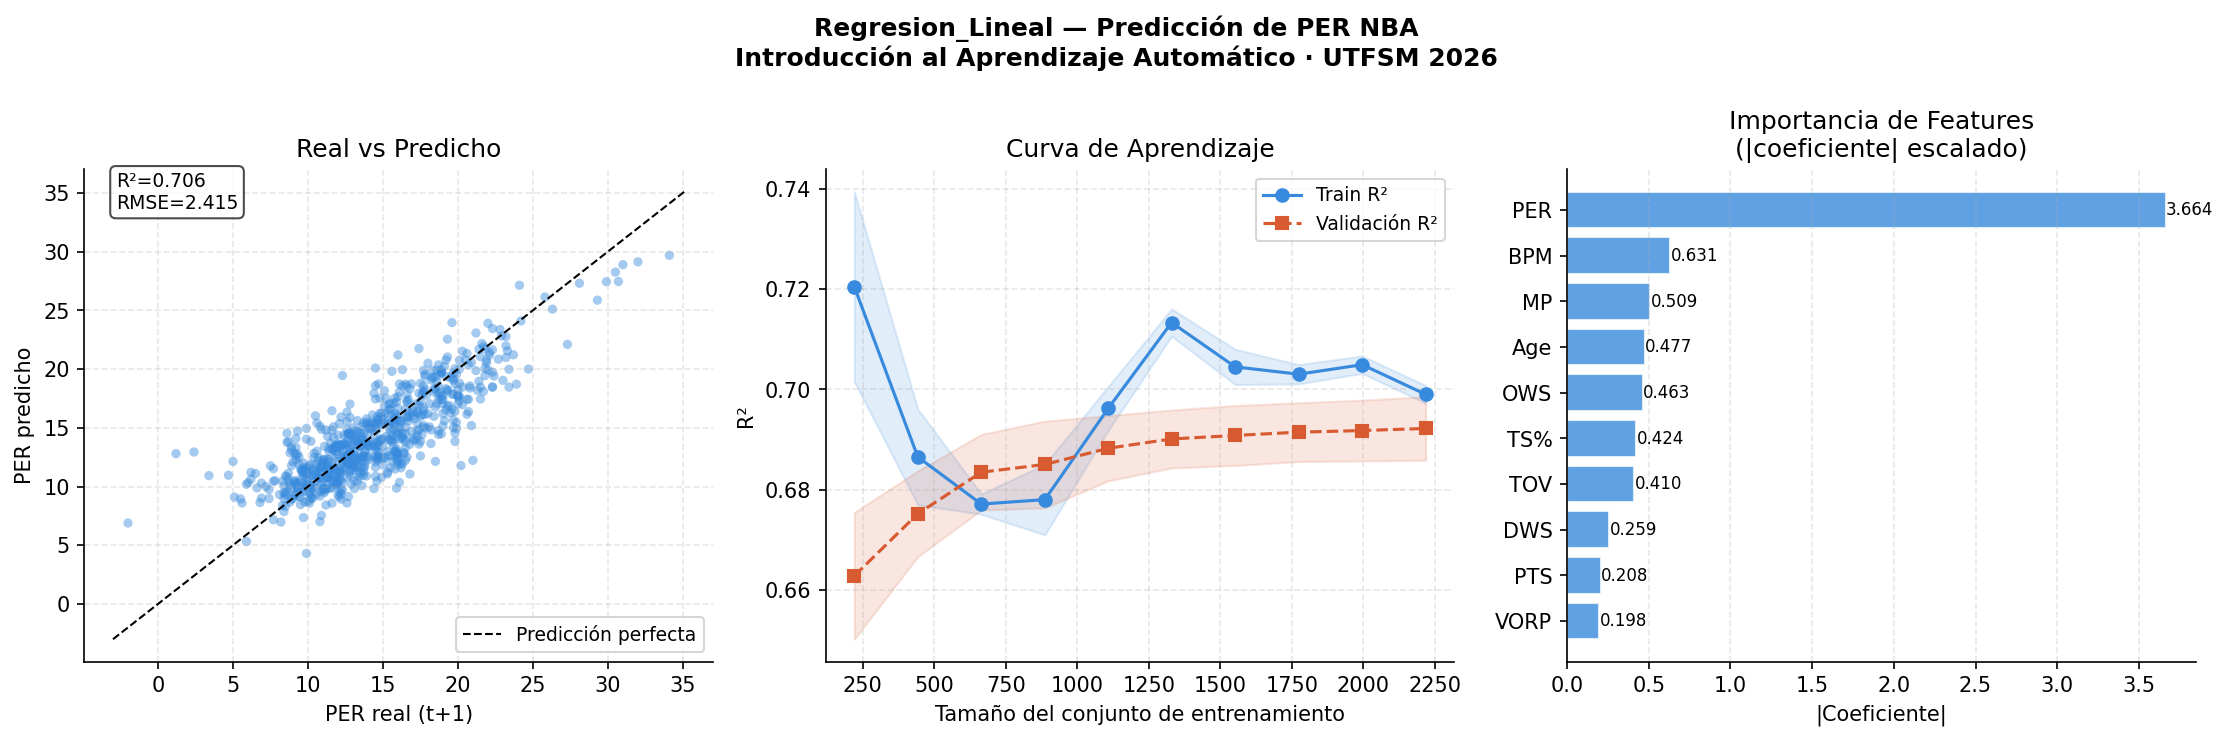
\includegraphics[width=0.95\textwidth]{Regresion_Lineal_resultados.png}
    \caption{Regresión Lineal (baseline): real vs.\ predicho, curva de
    aprendizaje e importancia de features por magnitud de coeficiente. El
    PER actual domina con coeficiente $\approx 3.66$, seguido de BPM, MP y
    Age.}
    \label{fig:lineal}
\end{figure}

Los cuatro modelos base convergen a un desempeño prácticamente idéntico
($R^2 \in [0.7047, 0.7063]$ en test), pese a tener capacidades muy
distintas desde un modelo lineal sin regularización hasta una red neuronal
con activaciones no lineales, lo que constituye la primera señal de un
posible techo con respecto a la informacion. Lasso identifica 13 de las 17 features como
relevantes, eliminando \texttt{DWS}, \texttt{PTS}, \texttt{AST} y \texttt{G}
por considerarlas redundantes frente a PER, WS y BPM.

\subsection{ Interacciones polinomiales}

\begin{figure}[H]
    \centering
    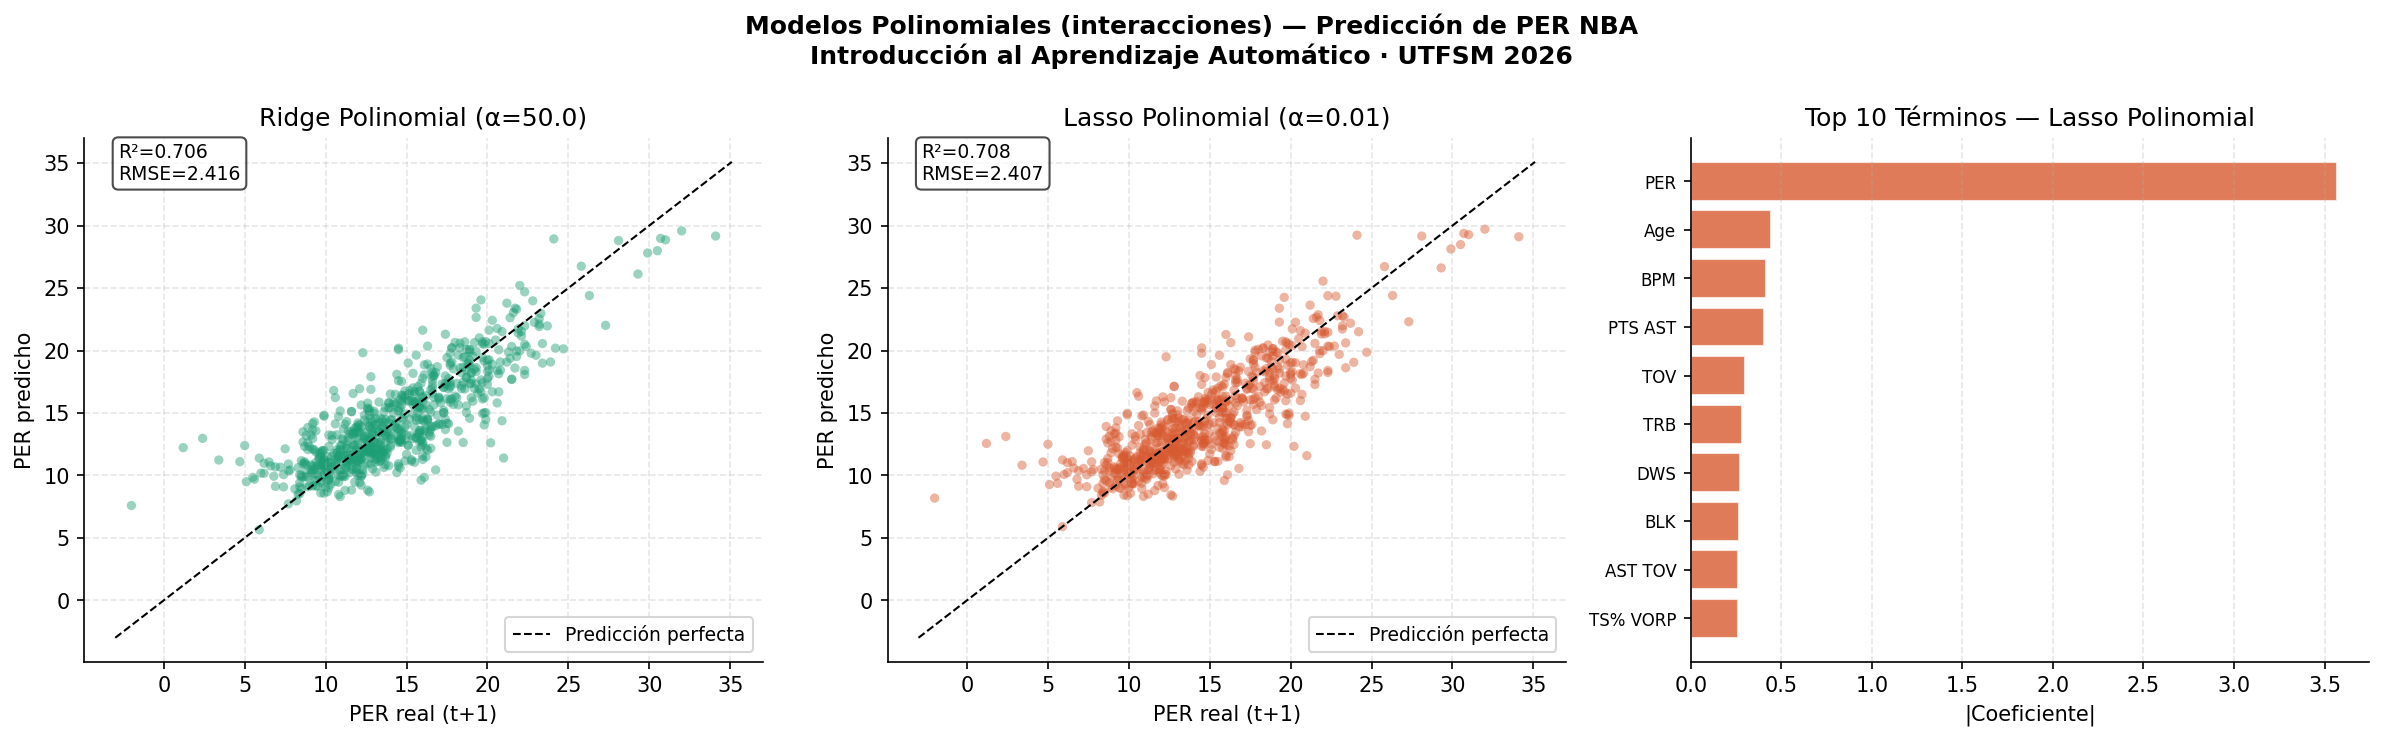
\includegraphics[width=0.95\textwidth]{Ridge_Lasso_Polinomial_resultados.png}
    \caption{Ridge y Lasso con 153 features (17 originales + interacciones
    de grado 2). Lasso Polinomial activa 74 de las 153 features, entre las
    interacciones más relevantes destaca $\text{PTS} \times \text{AST}$.}
    \label{fig:polinomial}
\end{figure}

Agregar interacciones de segundo grado  como $\text{USG\%} \times \text{TS\%}$,
$\text{PTS} \times \text{AST}$, entre otras. Se produce una mejora marginal, ya que
Lasso Polinomial alcanza $R^2=0.7081$, apenas 0.0034 por encima de su
versión sin interacciones. La interacción $\text{PTS} \times \text{AST}$
emerge como la tercera variable más relevante del modelo, sugiriendo que el
efecto combinado de anotar y repartir juego aporta información que ninguna
de las dos estadísticas captura por separado, aunque el efecto agregado
sobre el desempeño es pequeño.

\subsection{Búsqueda exhaustiva de hiperparámetros (MLP)}

Se evaluaron 32 combinaciones de arquitectura, regularización $\alpha$ y
tasa de aprendizaje mediante
\texttt{GridSearchCV}. El resultado más relevante de este bloque es
negativo, dado que la combinación óptima encontrada
($(64,32)$, $\alpha=0.0001$, \texttt{lr}=0.001) reproduce exactamente el
mismo Test $R^2=0.7047$ que la configuración por defecto usada en el
modelo base, indicando que el MLP ya operaba cerca de su techo de capacidad
para este conjunto de features, independientemente del ajuste  de sus
hiperparámetros internos.

\subsection{MLP mejorado (\texttt{lbfgs} + ensamble)}

\begin{figure}[H]
    \centering
    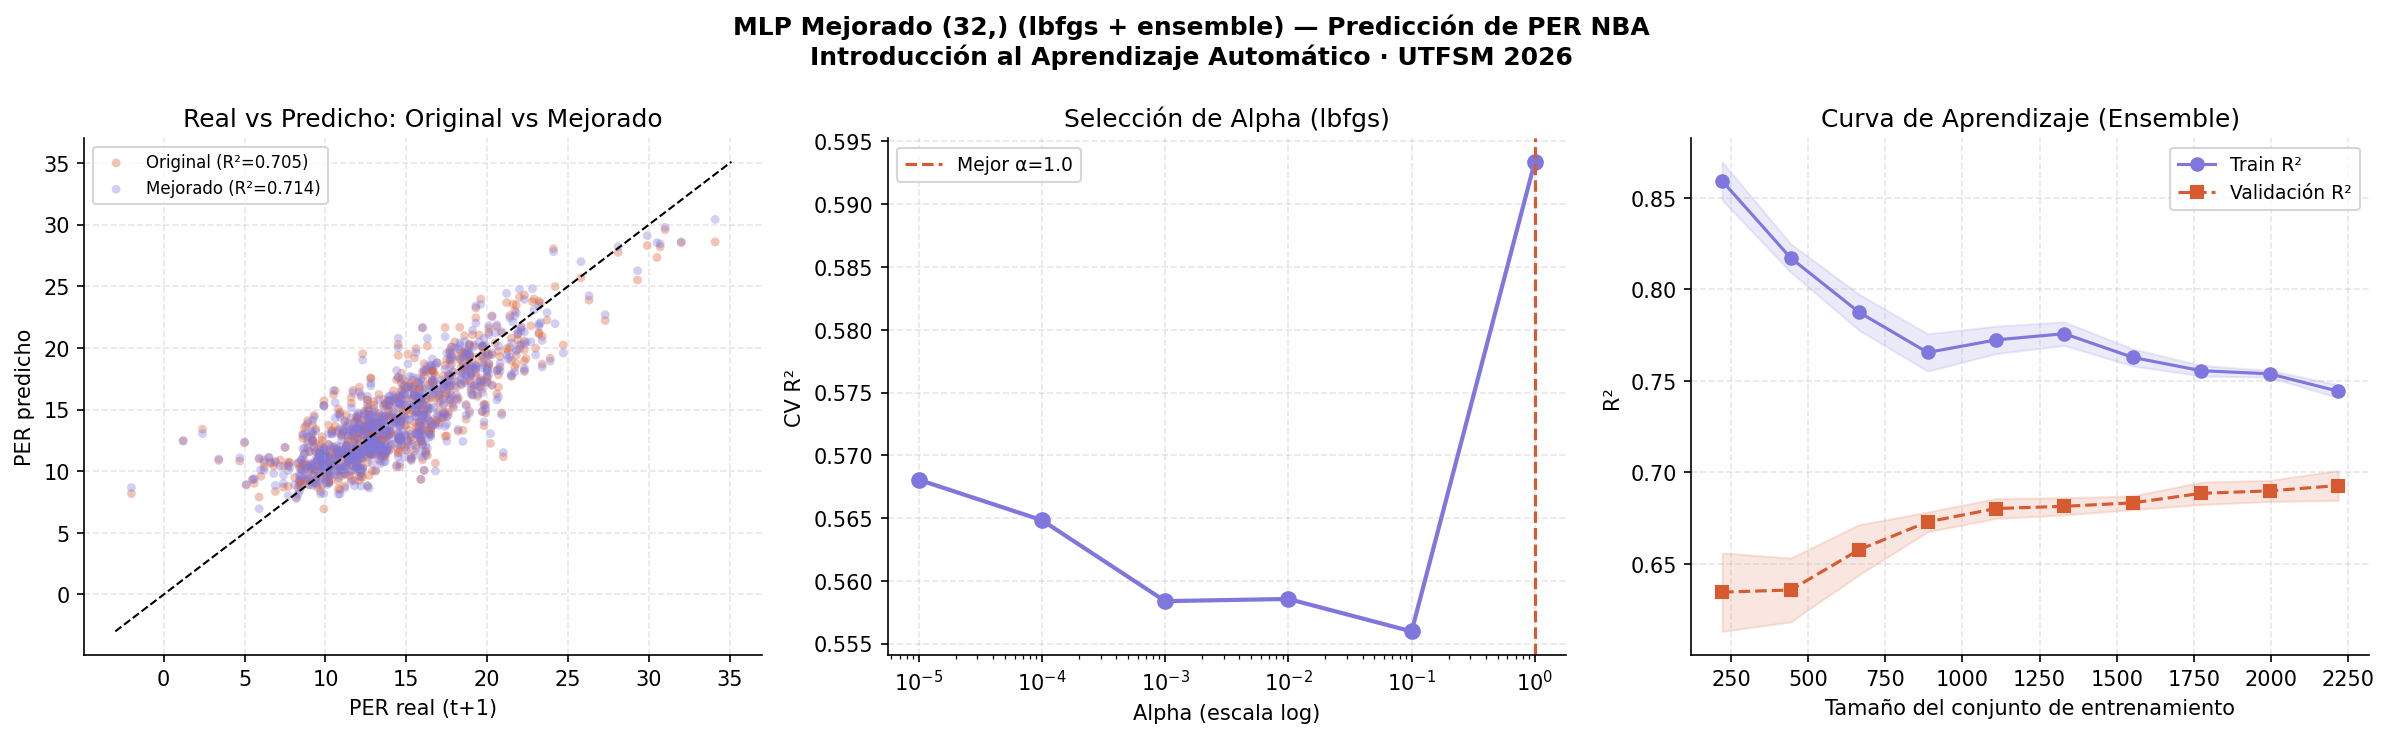
\includegraphics[width=0.95\textwidth]{MLP_Feedforward_v2_resultados.png}
    \caption{Comparación MLP original (\texttt{adam}) vs.\ mejorado
    \texttt{lbfgs}, sin early stopping, ensamble de 10 redes con
    semillas distintas. La mejora ($R^2$: $0.705 \to 0.714$) se explica
    por la reducción de varianza, no por mayor capacidad
    predictiva.}
    \label{fig:mlp_mejorado}
\end{figure}

Cambiar el optimizador a lbfgs y promediar las predicciones de 10
redes con distinta inicialización aleatoria produjo una mejora de
$+0.009$ en Test $R^2$ respecto al MLP original. Esta ganancia es
consistente con una reducción de varianza de inicialización más que con
una mayor capacidad de capturar señal, hipótesis que es reforzada por el hecho de
que un solo MLP con lbfgs mostró, durante la búsqueda de
hiperparámetros, un desempeño muy inestable, con un $R^2$ entre $0.555$ y
$0.595$ según el $\alpha$ probado que solo se estabiliza al promediarse
en el ensamble.

\subsection{Features temporales}

\begin{figure}[H]
    \centering
    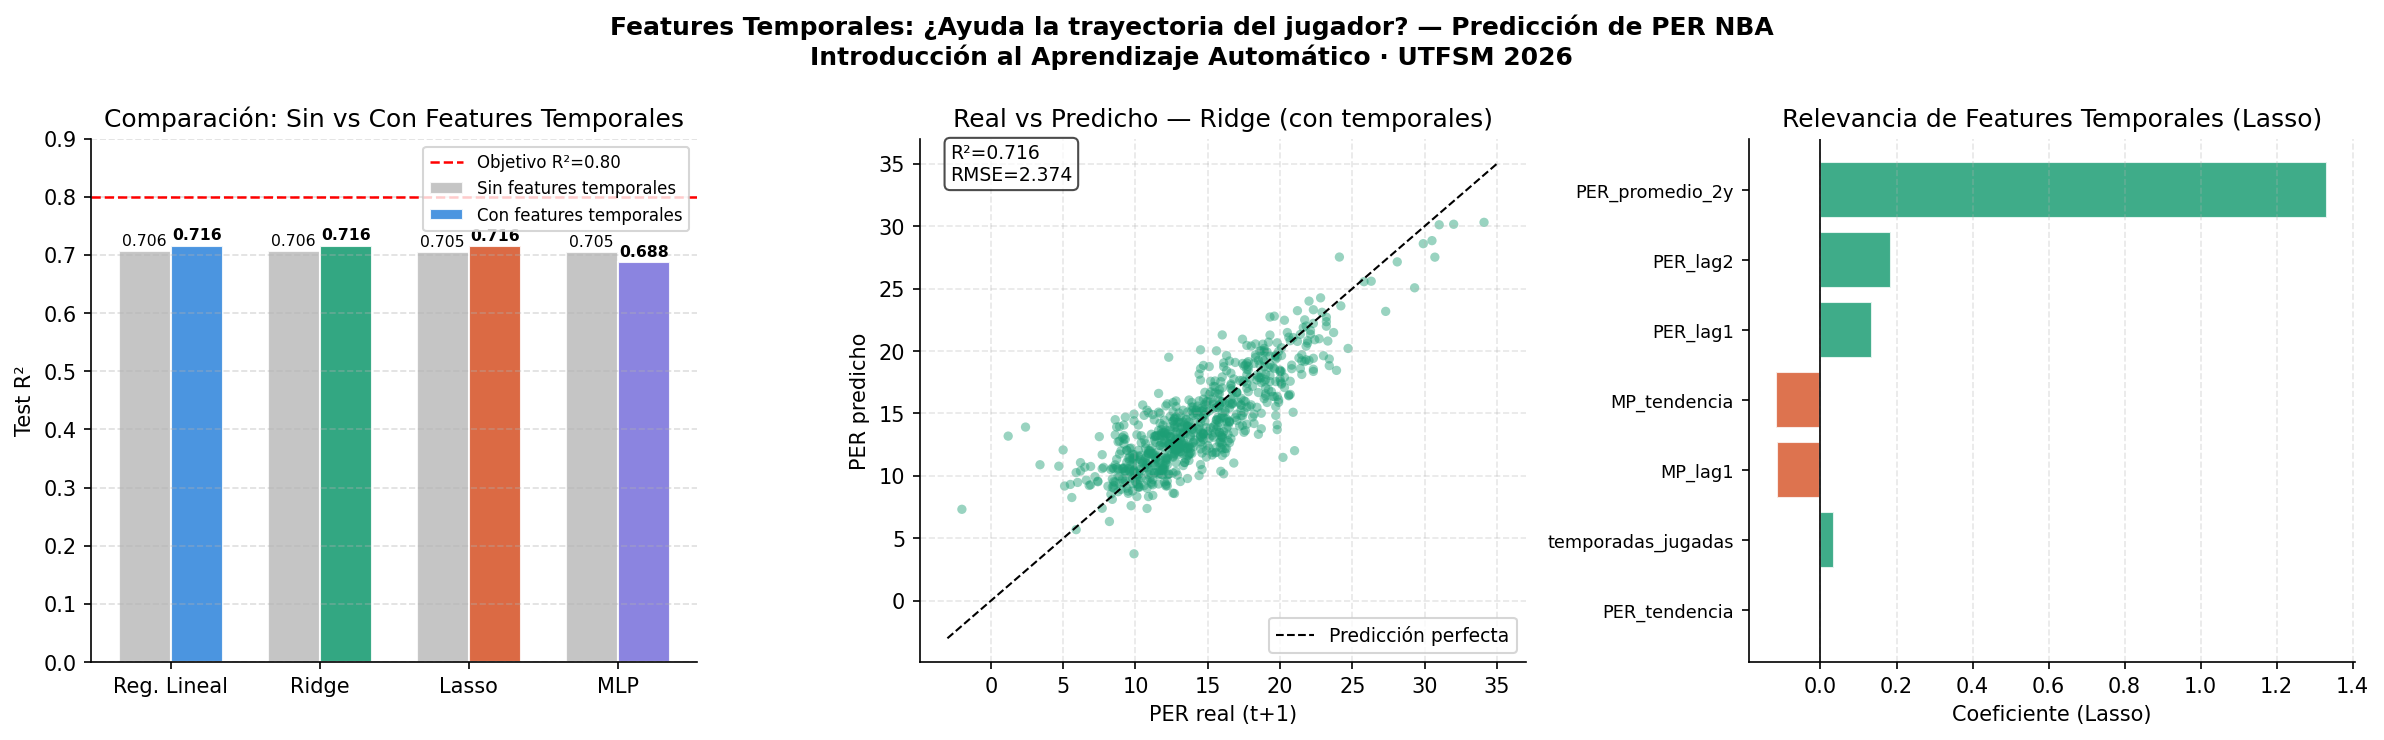
\includegraphics[width=0.95\textwidth]{Features_Temporales_resultados.png}
    \caption{Comparación sin/con features temporales para los 4 modelos, real vs.\ predicho del mejor modelo del proyecto,
    Ridge + temporal, relevancia de las 7 features
    temporales según los coeficientes de Lasso.}
    \label{fig:temporales}
\end{figure}

Se incorporaron features que dan al modelo visibilidad de la trayectoria
del jugador, no solo su última temporada, PER y minutos jugados de 1 y 2
temporadas atrás, tendencia, promedio móvil de 2 años, y temporadas
acumuladas en el dataset. Los tres modelos lineales mejoran de forma
consistente y simultánea,
el único caso donde una modificación beneficia
a Regresión Lineal, Ridge y Lasso a la vez. El hallazgo más
notable es que PER\_promedio\_2y obtiene el coeficiente de mayor
magnitud de todo el proyecto ($1.33$), superando incluso al PER
de la temporada actual en los modelos sin features temporales —sugiriendo
que un promedio suavizado de dos años predice mejor el futuro que el valor
de una sola temporada, posiblemente al reducir el ruido de temporadas
atípicas.

El MLP, en cambio, es el único modelo que empeora con las
features temporales, $R^2$: $0.7047 \to 0.6881$, resultado que se puede deber al
aumento de dimensionalidad sobre un conjunto de
entrenamiento de tamaño fijo, combinado con la alta multicolinealidad
entre las nuevas features temporales del PER algo que los modelos lineales
regularizados manejan mejor por diseño que una red neuronal sin ese
mecanismo explícito.

% ─────────────────────────────────────────────────────────────────────────────
\section{Análisis Crítico de los Resultados}
% ─────────────────────────────────────────────────────────────────────────────

El hallazgo central del proyecto es que, a través de las variantes
de modelo evaluadas en 5 bloques experimentales distintos —desde
regresión lineal simple hasta optimización exhaustiva de hiperparámetros,
interacciones no lineales y contexto temporal, el desempeño se mantiene
acotado en una banda estrecha de $R^2 \in [0.688, 0.716]$, muy por debajo
del objetivo de $R^2 > 0.80$ planteado al inicio del proyecto.

Esta convergencia, no debe ser considerado como un fracaso, ya que constituye
evidencia sólida en favor de la hipótesis
informacional, el límite no proviene de una elección subóptima de modelo
o de hiperparámetros, sino de la información contenida en las estadísticas
de Basketball-Reference.

\begin{enumerate}[leftmargin=*, itemsep=5pt]
    \item \textbf{Insensibilidad a la capacidad del modelo.} El MLP es el único modelo no lineal y nunca superó de forma consistente a los
    modelos lineales regularizados, ni siquiera tras 160 evaluaciones de
    \texttt{GridSearchCV} y mejoras específicas de optimización.
    Si existiera una relación no lineal fuerte sin explotar,
    se esperaría que el MLP la capturara y se despegara claramente de
    Ridge y Lasso.

    \item \textbf{Rendimientos decrecientes en intervenciones costosas.}
    Las interacciones polinomiales (153 features) y la búsqueda
    exhaustiva de hiperparámetros (160 entrenamientos) ambas
    muy costosas a nivel computacional produjeron mejoras de $0.001$-$0.003$ en
    $R^2$, mientras que agregar 3 features temporales simples
    produjo una mejora de $0.009$--$0.011$, casi un orden de magnitud
    mayor con una fracción del costo computacional. Esto sugiere que el
    problema no carecía de capacidad de modelado, sino de
    información relevante en las features originales.

    \item \textbf{Consistencia con la literatura.} El mejor resultado
    obtenido  siende este $R^2=0.7159$ es comparable al reportado por
    Nguyen et al.~\cite{nguyen2022} para problemas afines en el mismo
    dominio, y notablemente superior al $R^2\approx 0.65$ de
    Seshadri~\cite{seshadri2024} con Lasso sobre PER directo. Ningún
    estudio revisado en la literatura reporta $R^2 > 0.80$ para predicción
    de rendimiento individual NBA usando exclusivamente estadísticas de
    caja (\textit{box score}).
\end{enumerate}

\subsection{Variables ausentes que explicarían el techo}

El componente de varianza no explicada ($\approx 30\%$) es mas
atribuible a factores no capturados por ninguna estadística considerada,
lesiones y su severidad, cambios de equipo o de rol táctico entre
temporadas, decisiones de entrenador, minutos asignados, posición en la
rotación, y la asincronía entre el peak de forma física de un jugador y
el calendario de temporadas. Estas variables no están disponibles en
las fuentes consultadas y representarían el camino más prometedor, aunque fuera
del alcance de este proyecto, para acercarse al objetivo de
$R^2 > 0.80$.

% ─────────────────────────────────────────────────────────────────────────────
\section{Conclusiones y Posible Trabajo Futuro}
\label{sec:futuro}
% ─────────────────────────────────────────────────────────────────────────────

Este proyecto evaluó distintas variantes de cuatro modelos de regresión
supervisada, para reiterar estos son Regresión Lineal, Ridge, Lasso y MLP con el objetivo de predecir el PER de
jugadores NBA en la temporada siguiente, explorando sistemáticamente
features de interacción, optimización exhaustiva de hiperparámetros,
mejoras de entrenamiento del MLP y features de contexto temporal.

El mejor modelo obtenido es Ridge Regression con features
temporales ($\alpha=5.0$), alcanzando $R^2=0.7159$ y $\text{RMSE}=2.3744$
en el conjunto de test, sin alcanzar el objetivo inicial de
$R^2 > 0.80$. El hallazgo principal del proyecto es que este techo de
desempeño es adecuado a la elección de modelo y a la sofisticación
de las técnicas aplicadas, lo que es evidencia de un límite
en la informacion recopilada en las estadísticas disponibles, más que una
limitación de los algoritmos elegidos.

Como hallazgos secundarios de valor, primero que las features temporales, destacando el promedio móvil de 2 años del PER resultaron más
informativas que cualquier transformación no lineal de las features de una
sola temporada, por otro lado, Lasso permite identificar de forma automática qué
estadísticas son redundantes (PTS, AST, DWS, G) frente a métricas
agregadas como PER, WS y BPM y, por ultimo, el MLP, pese a su mayor capacidad
teórica, fue notoriamente el modelo más sensible al aumento de
dimensionalidad y a la multicolinealidad entre features.

\subsection*{Trabajo futuro}

Como opcion abierta a la continuacion del proyecto, se puede:

\begin{itemize}[leftmargin=*, itemsep=4pt]
    \item Incorporar variables externas no presentes en las fuentes consultadas como historial de lesiones, cambios de equipo o minutos proyectados por el
    cuerpo técnico para evaluar si reducen la varianza no explicada.

    \item Entrenar versiones de cada modelo excluyendo el PER
    actual de las features, para descartar que esta variable domine de
    forma artificial la predicción y oculte el aporte real del resto
    de las estadísticas.

    \item Evaluar un modelo de ensemble explícito que
    combine las predicciones de Ridge, Lasso y MLP, en lugar de evaluarlos
    de forma independiente.

    \item Extender el análisis segmentando por posición o por rango
    de PER, para evaluar si el desempeño del modelo varia entre
    subgrupos de jugadores.
\end{itemize}

% ─────────────────────────────────────────────────────────────────────────────
\begin{thebibliography}{9}

\bibitem{seshadri2024}
Seshadri, R. (2024).
\textit{Improving Player Efficiency Rating in Basketball through Machine
Learning}.
Research Archive of Rising Scholars (preprint).
DOI: \href{https://doi.org/10.55223/axbxc.221}{10.55223/axbxc.221}

\bibitem{nguyen2022}
Nguyen, N.~H., Nguyen, D.~T.~A., Ma, B., \& Hu, J. (2022).
\textit{The application of machine learning and deep learning in sport:
predicting NBA players' performance and popularity}.
Journal of Information and Telecommunication, 6(2), 217--235.
DOI: \href{https://doi.org/10.1080/24751839.2021.1977066}{10.1080/24751839.2021.1977066}

\bibitem{loeffelholz2009}
Loeffelholz, B., Bednar, E., \& Bauer, K.~W. (2009).
\textit{Predicting NBA Games Using Neural Networks}.
Journal of Quantitative Analysis in Sports, 5(1).
DOI: \href{https://doi.org/10.2202/1559-0410.1156}{10.2202/1559-0410.1156}

\bibitem{terner2021}
Terner, Z., \& Franks, A. (2021).
\textit{Modeling Player and Team Performance in Basketball}.
Annual Review of Statistics and Its Application, 8, 1--23.
DOI: \href{https://doi.org/10.1146/annurev-statistics-040720-015536}{10.1146/annurev-statistics-040720-015536}

\bibitem{miljkovic2010}
Miljković, D., Gajić, L., Kovačević, A., \& Konjović, Z. (2010).
\textit{The use of data mining for basketball matches outcomes prediction}.
IEEE 8th International Symposium on Intelligent Systems and Informatics
(SISY), pp. 309--312.
DOI: \href{https://doi.org/10.1109/SISY.2010.5647440}{10.1109/SISY.2010.5647440}

\bibitem{sarlis2020}
Sarlis, V., \& Tjortjis, C. (2020).
\textit{Sports analytics --- Evaluation of basketball players and team
performance}.
Information Systems, 93, 101562.
DOI: \href{https://doi.org/10.1016/j.is.2020.101562}{10.1016/j.is.2020.101562}

\end{thebibliography}

\end{document}